\chapter{云端根因诊断与反馈闭环}

\section{从单事件到关联上下文}
边缘推理擅长在低时延条件下处理单条或局部事件，云端诊断的价值则来自更强的语义能力与更完整的上下文。\texttt{cloud-gateway} 围绕主事件，从近期边缘事件中按照时间、模板、来源、设备、类别和严重度选择相关记录，并在 Token 预算内裁剪。它不是无边界地拼接全部日志，而是组织一份与当前问题直接相关的诊断材料。

时间邻近可以提示故障传播顺序，相同设备或模板可以提示重复模式，跨来源的高严重度事件则可能指向共同依赖故障。上云前，系统对主事件和关联事件的原始日志执行常见敏感模式脱敏；进一步工程化还需将模板、设备、来源和其他提示字段纳入统一字段级策略。

\section{异常态势与云端深诊}
\begin{figure}[htbp]
  \centering
  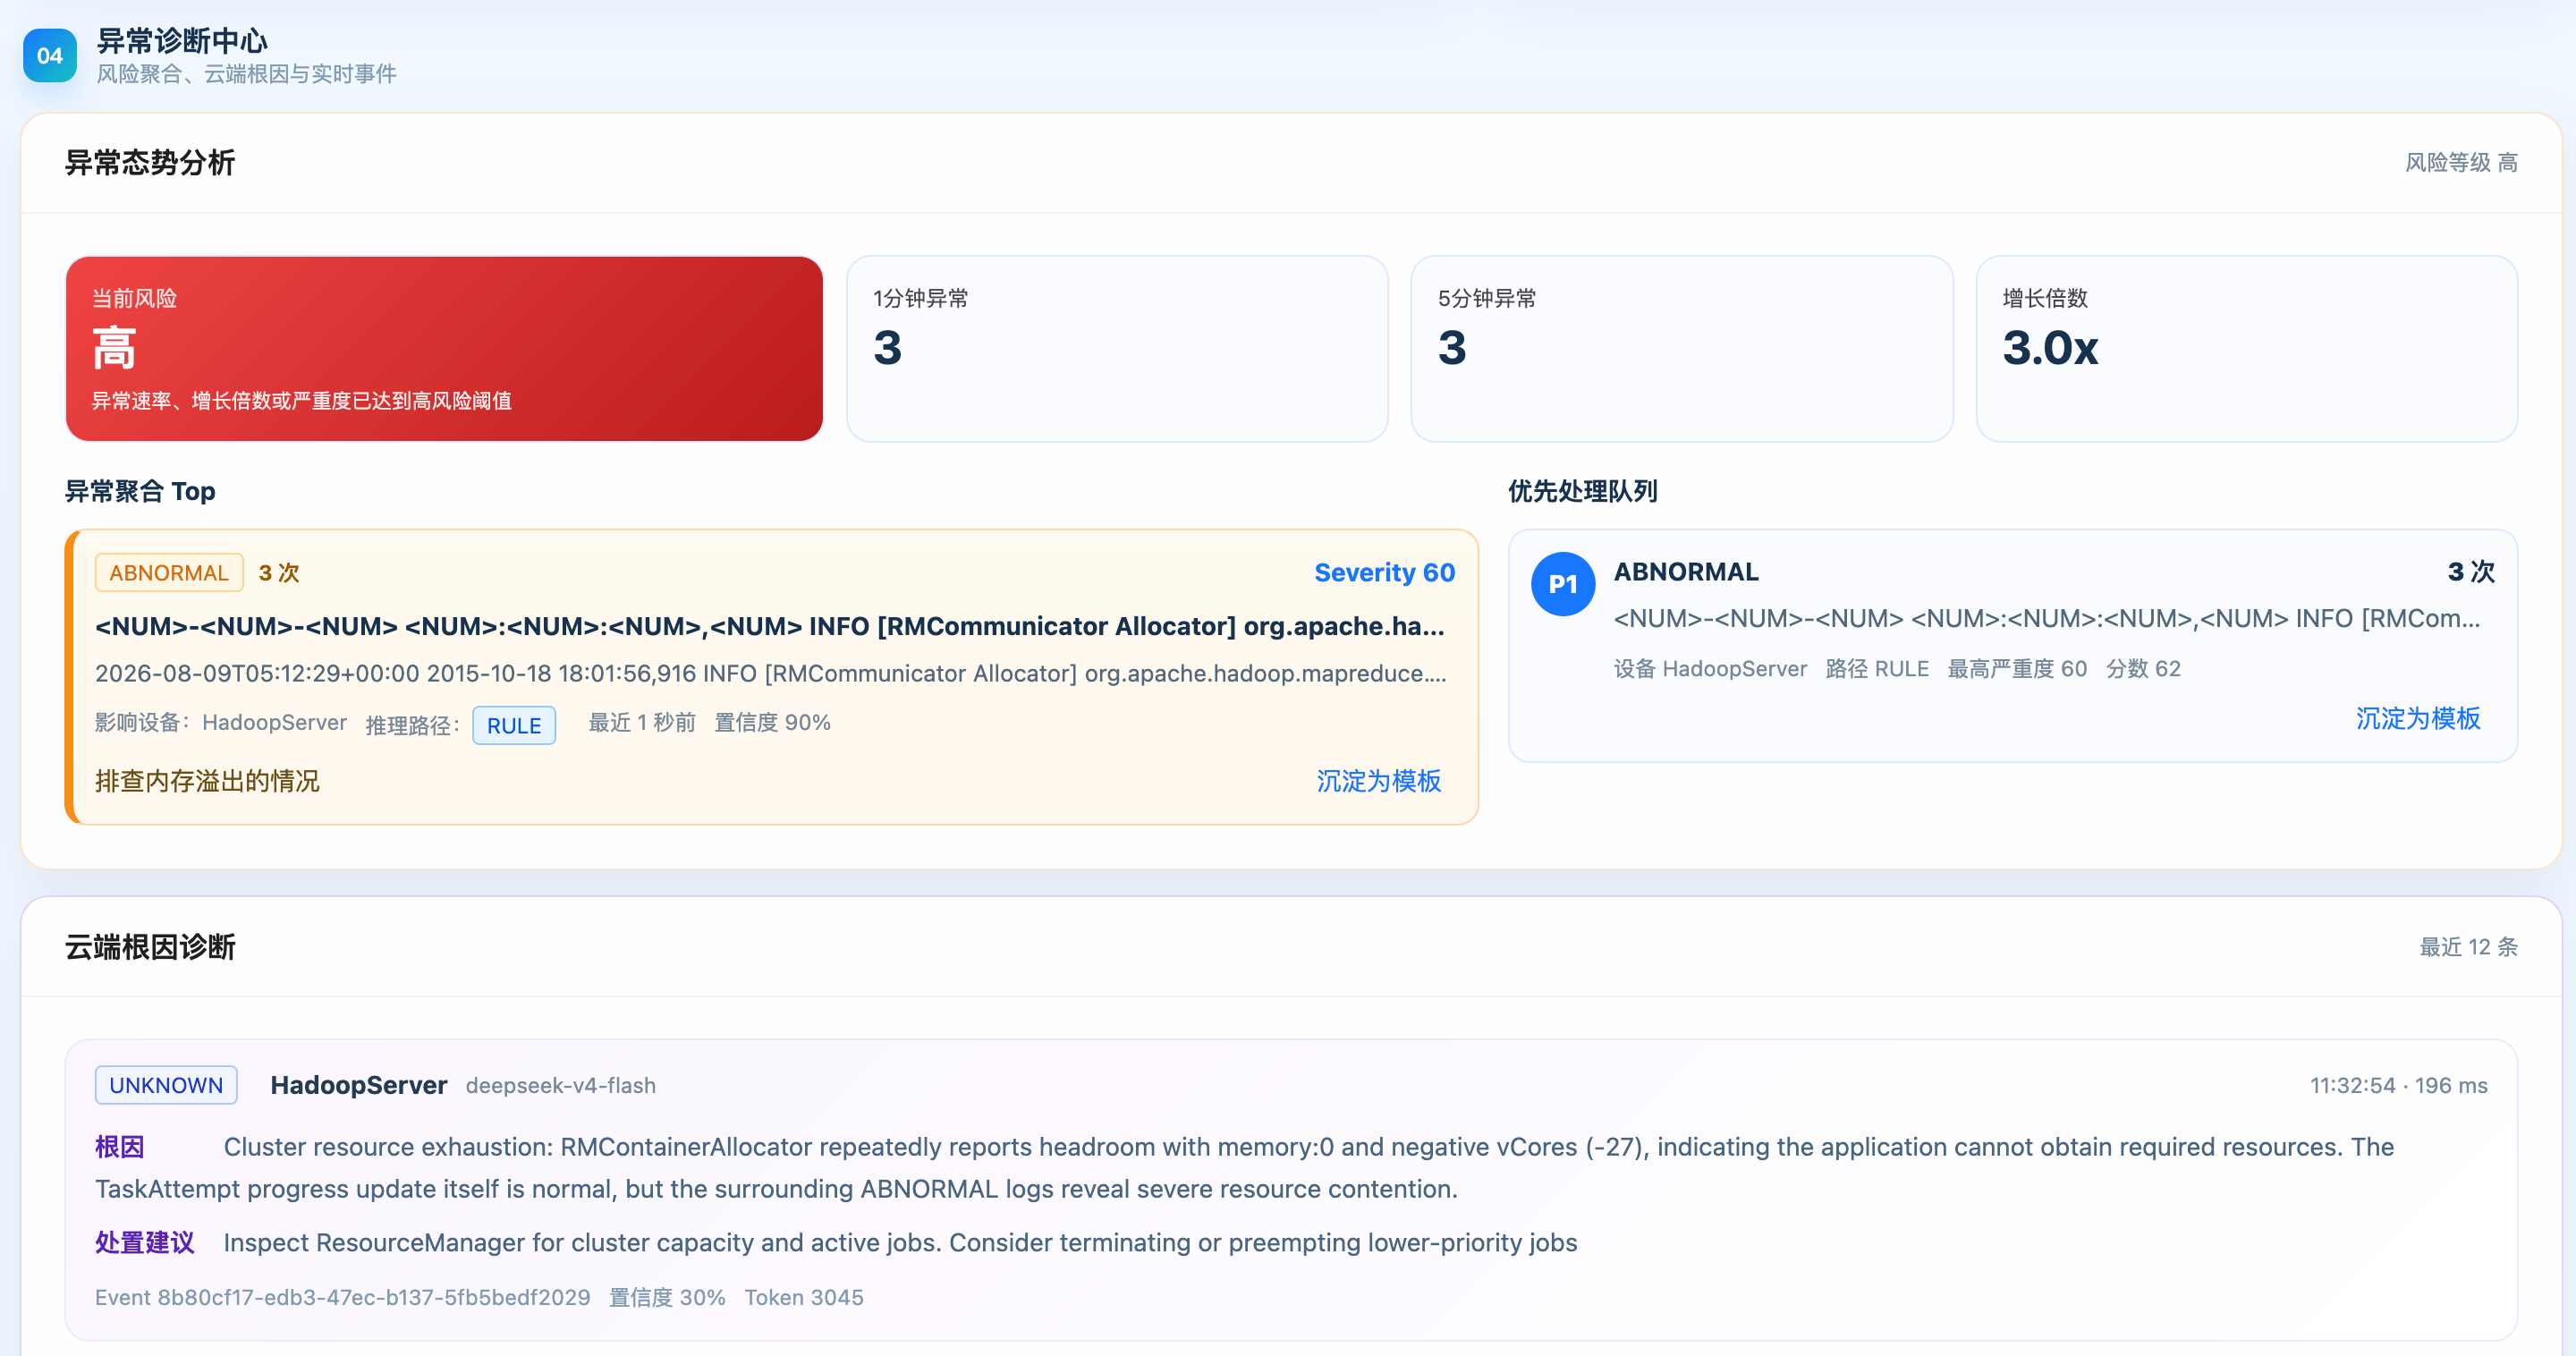
\includegraphics[width=0.98\textwidth]{figures/s-03b-anomaly-diagnosis-center-overview.png}
  \caption{异常态势、优先队列与云端根因诊断的统一界面}
  \label{fig:diagnosis-center}
\end{figure}

\cref{fig:diagnosis-center}把异常趋势、风险聚合、优先处理队列、云端根因诊断和实时事件放在同一页面中。运维人员可以先从总体风险发现问题，再沿具体事件下钻到诊断结果。页面中边缘字段与云端字段属于不同处理阶段，不应仅凭标签差异计算判断准确率或冲突解决效果。

\begin{figure}[htbp]
  \centering
  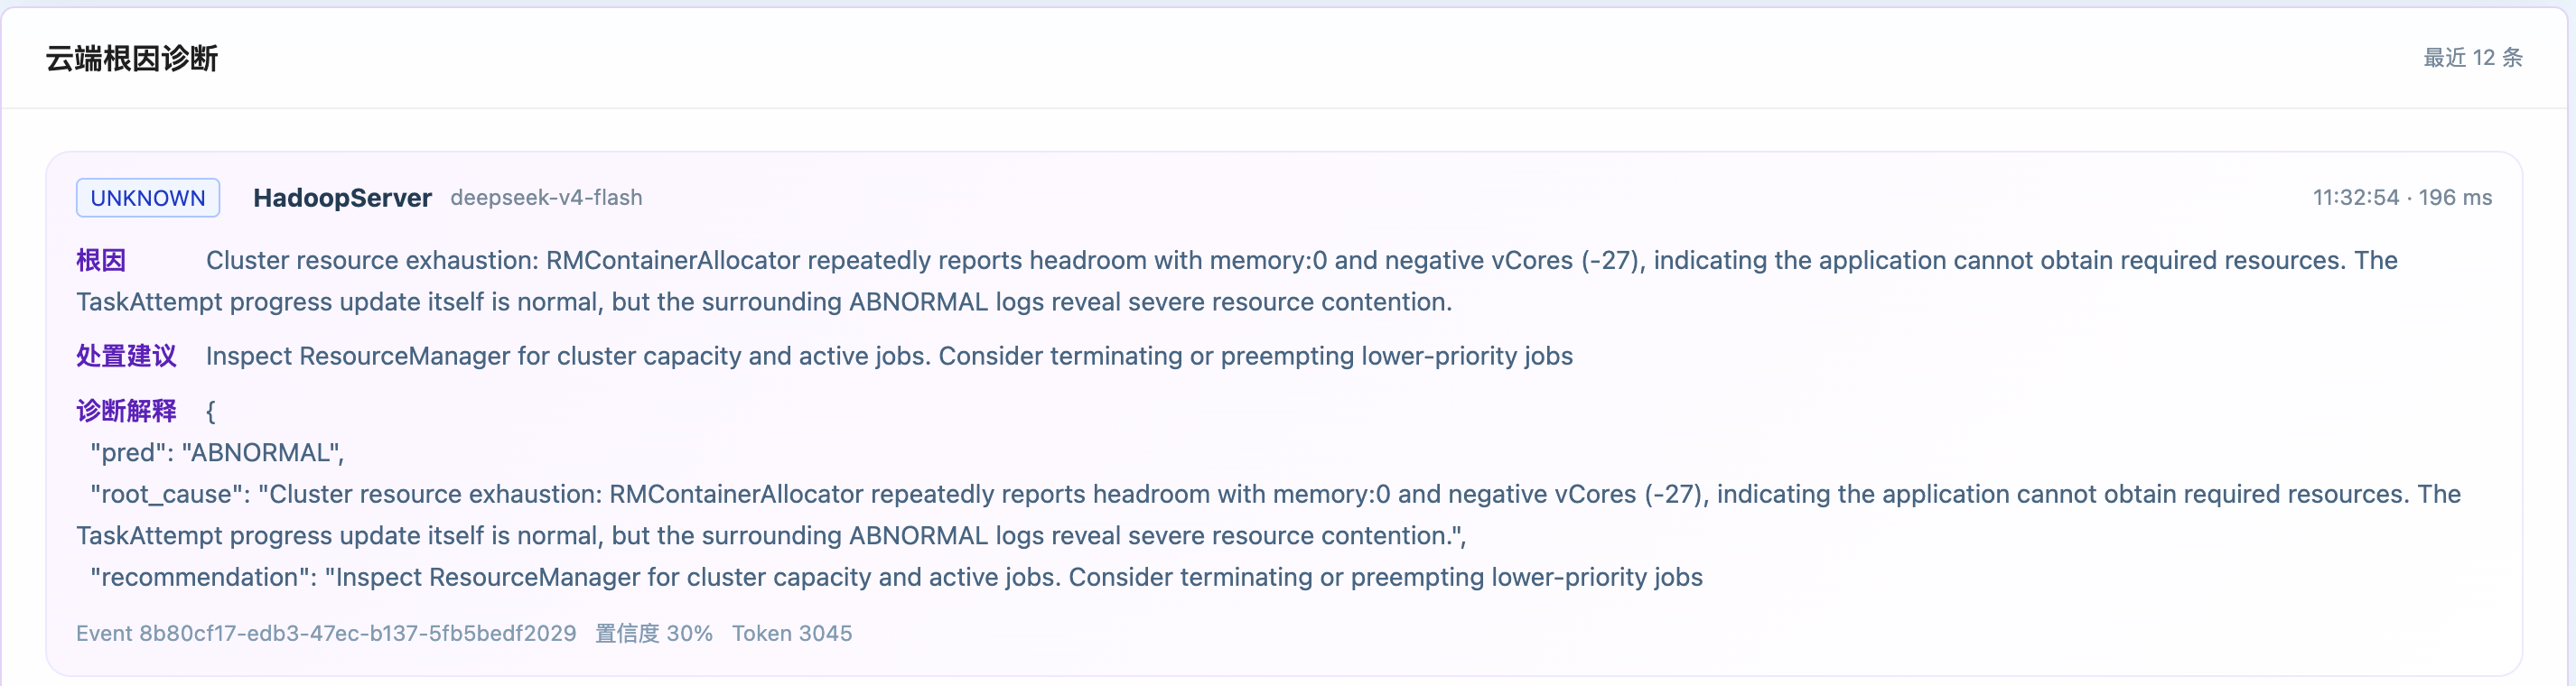
\includegraphics[width=0.98\textwidth]{figures/s-05a-cloud-root-cause-diagnosis.png}
  \caption{云端结构化根因、处置建议与诊断解释}
  \label{fig:cloud-root-cause-diagnosis-v03}
\end{figure}

\cref{fig:cloud-root-cause-diagnosis-v03}展示了单条云端诊断的详细形态。系统不仅呈现一个类别，还同时保留模型信息、根因候选、处置建议、结构化解释、置信度、Token 用量与处理时延，使“发生了什么”“为什么这样判断”“下一步可以做什么”能够在同一结果中被阅读。

\section{结构化输出与降级解析}
云端模型的理想输出是稳定 JSON，但真实 Provider 可能返回被代码块包裹的 JSON、夹杂说明文本的对象，甚至完全非结构化的内容。网关因此采用分级解析：优先严格解析完整对象，其次提取文本中的对象片段，仍无法解析时保留原文并进入明确降级路径。主要字段如\cref{tab:cloud-output}所示。

\begin{table}[htbp]
  \centering
  \small
  \caption{云端诊断输出及其运维用途}
  \label{tab:cloud-output}
  \begin{tabularx}{\textwidth}{>{\ttfamily}p{0.22\textwidth} X X}
    \toprule
    \normalfont\bfseries 字段 & \textbf{含义} & \textbf{界面用途} \\
    \midrule
    pred / confidence & 云端复判类别及把握程度 & 与边缘初判并列查看 \\
    root\_cause & 结合关联上下文形成的根因候选 & 支持故障定位与影响分析 \\
    recommendation & 面向运维人员的处置建议 & 连接诊断与后续行动 \\
    explanation & 结构化诊断依据或原始解析内容 & 支持审阅、追踪与降级展示 \\
    latency / token & 本次调用时延与 Token 用量 & 进入运行成本和性能观测 \\
    \bottomrule
  \end{tabularx}
\end{table}

\section{幂等写回与在线反馈}
云端结果先依据幂等键写入 MySQL，再发布响应通知，最后确认请求消息。如果持久化已经完成而通知失败，重试可以复用既有结果，避免再次调用云端模型。该顺序把高成本调用置于幂等边界内，降低重复计费和结果漂移风险。

反馈处理会根据云端是否纠正边缘判断、是否补充根因与建议、是否确认高风险事件等信号更新模板统计、探索状态和 GainModel 快照。当前已学习增益尚未直接进入 RAISE 决策分数，两阶段 Reward 的语义也需要进一步统一。因此，现阶段更准确的定位是“具有结构化反馈和在线统计的动态路由”，而不是已经由反馈完全自适应的闭环。反馈公式及其与在线评分的衔接方式见第 6 章。

\section{从诊断到业务处置}
核心仓库将结构化结果保存并开放给查询与展示接口，不内置生产现场的自动处置执行器。实际落地时，可由告警平台、工单系统或设备控制系统订阅本地和云端结果，并根据自身权限与安全策略执行后续动作。这样既避免诊断系统越权控制生产设备，也为不同企业的处置流程保留接入空间。
